\documentclass[11pt]{article}
\usepackage[margin=1in]{geometry}
\usepackage{amsmath,amssymb,amsthm,mathtools,booktabs,longtable,array,microtype}
\usepackage{enumitem,xcolor,tikz,fvextra,fontspec}
\IfFontExistsTF{DejaVu Sans Mono}
  {\newfontfamily\leanmono[NFSSFamily=LeanMono]{DejaVu Sans Mono}}
  {\newfontfamily\leanmono[NFSSFamily=LeanMono]{Menlo}}
\fvset{fontfamily=LeanMono,fontsize=\scriptsize,breaklines=true,breakanywhere=true,
  frame=single,rulecolor=\color{black!20}}
\usetikzlibrary{arrows.meta,positioning}
\usepackage[colorlinks=true,linkcolor=blue!55!black,urlcolor=blue!55!black]{hyperref}
\usepackage{url}
\newtheorem{definition}{Definition}[section]
\newtheorem{theorem}[definition]{Theorem}
\newtheorem{example}[definition]{Example}
\newtheorem{counterexample}[definition]{Counterexample}
\newcommand{\eqE}{\mathrel{=_{E}}}
\newcommand{\enc}{\mathsf{penc}}
\newcommand{\pk}{\mathsf{pk}}
\newcommand{\spk}{\mathsf{spk}}
\newcommand{\checkspk}{\mathsf{checkspk}}
\newcommand{\dec}{\mathsf{dec}}
\newcommand{\pd}{\mathsf{partialDecrypt}}
\newcommand{\Pub}{\mathsf{Public}}
\newcommand{\Acc}{\mathsf{Accepted}}
\newcommand{\NF}{\mathsf{NoncesFreshFor}}
\newcommand{\Cand}{\mathsf{CandidateValues}}
\newcommand{\W}{\mathcal E}
\newcommand{\code}[1]{\texttt{\detokenize{#1}}}
% Anchors are parsed by the citation gate. Paths are relative to Helios/.
\newcommand{\anchor}[2]{\par\vspace{2pt}{\footnotesize\noindent
  Lean: \href{../../ExplainableCrypto/Helios/#1.lean}{\nolinkurl{#2}}.\par}\vspace{1pt}}
\newcommand{\companchor}[2]{\par\vspace{2pt}{\footnotesize\noindent
  Lean: \href{../../ExplainableCrypto/Helios/Computational/#1.lean}{\nolinkurl{#2}}.\par}\vspace{1pt}}
\setlist{nosep,leftmargin=*}
\setlength{\emergencystretch}{2em}
\tikzset{box/.style={draw=blue!55!black,rounded corners,fill=blue!3,
  align=center,text width=4.5cm,inner sep=6pt},
  arrow/.style={-{Latex[length=2mm]},semithick}}
\title{Helios: Protocol, Attacks, Repair\\and Scoped Ballot Secrecy\\[5pt]
  \large Formal reference to the Lean development}
\author{KC Sivaramakrishnan\\FP Launchpad, IIT Madras}
\date{16 September 2026}
\hypersetup{pdftitle={Helios Formal Reference},pdfauthor={KC Sivaramakrishnan},
  bookmarksopen=true,bookmarksnumbered=true}
\begin{document}
\maketitle
\begin{abstract}
This reference explains the historical homomorphic Helios protocol, the replay
and permutation attacks, component weeding, and the Lean proof of
symbolic ballot secrecy for the documented repair. It connects the mathematical
objects to their public declarations and organizes the proof by semantic
dependency. Applied-pi-calculus infrastructure and symbolic homomorphic
computation are treated as verified project-local libraries through their
interfaces. Their internal proofs are outside the exposition. A concrete
probabilistic attack, repair, finite DDH reduction and parameterized secrecy
theorem are also checked. The computational endpoint retains explicit attacker
resource conditions and external implementation/efficiency arguments. The models
have separately documented scopes; no symbolic-to-computational correspondence
or general transfer theorem has been proved.
\end{abstract}
{\setcounter{tocdepth}{1}\footnotesize\tableofcontents}


\section*{Reading this reference}
The protocol and symbolic observation model come first, followed by symbolic
secrecy, concrete cryptographic algorithms, the probabilistic attack and repair,
and computational secrecy. The two results have different scopes: the symbolic
repair and observation schedule are not identified with the computational game.
Section~\ref{sec:scope-comparison} lists the differences.
For a computational reading, start with Sections~\ref{sec:concrete}--\ref{sec:computational-final}
(algorithms, attack, repair and secrecy), then read
Sections~\ref{sec:scope-comparison} and~\ref{sec:future} for the scope comparison
and limitations. Sections~\ref{sec:protocol}--\ref{sec:controls} develop the symbolic model.

Mathematical displays are transcriptions or explicitly labelled compressions of
linked Lean declarations. Symbolic candidate indices are one-based in the text;
Lean uses zero-based finite indices. $\eqE$ denotes equality in the symbolic
equational theory, while ordinary $=$ denotes mathematical equality. The
protocol provenance is Cortier--Smyth's historical homomorphic Helios description,
especially \S5 and Figure~4~\cite{cs}, with the tuple correction stated below.

Lean checks the proofs under the cited definitions. The axiom audit accepts
\code{propext}, \code{Classical.choice}, and \code{Quot.sound}; it does not
certify the prose transcription, external efficiency arguments, or fidelity to
deployed software. The separate \href{catalogue.pdf}{historical development
catalogue} records supporting component constructions from source revision
\code{9273cdc}.
It is supplementary to the mathematical argument here.
\clearpage
\section{Election, ballots and public transcript}\label{sec:protocol}
There are $\ell=n+1>0$ candidates, two honest voters, a bulletin board, a
trustee and $q\in\mathbb N$ additional voter inputs. The honest voters submit
first, on restricted channels. The board publishes their ballots in order.
Subsequent inputs use separate public voter channels and are checked against
all preceding accepted ballots. The board and trustee follow the specified
programs. The theorem concerns one such finite election for every $q$.

Let $k$ be the secret key, $K=\pk(k)$ the public key, and $r_{ij}$ the
fresh nonce for honest voter $i\in\{0,1\}$ and candidate $j$. A vote is a
vector of ground symbolic terms $v=(v_1,\ldots,v_\ell)$ satisfying
\[
  \Cand(v)\quad\Longleftrightarrow\quad
  \sum_{j=1}^{\ell}v_j\eqE 0\ \lor\
  \sum_{j=1}^{\ell}v_j\eqE 1.
\]
The sum is a nonempty fold of symbolic addition. This condition entails that
each component is $E$-equal to zero or one. It permits arbitrary equivalent
term representatives, including the all-zero abstention vector.
\anchor{Symbolic/BallotValues}{CandidateValues}
\anchor{Symbolic/CandidateSubstitutions}{CandidateSubstitution.bit_representative}

\begin{definition}[Honest ballot; notation-level transcription]
For voter $i$ with vector $v$, define
\begin{align*}
 c_{ij}&=\enc(K,r_{ij},v_j),&
 p_{ij}&=\spk(K,r_{ij},v_j,c_{ij}),\\
 C_i&=\prod_{j=1}^{\ell}c_{ij},&
 R_i&=\mathop{\circ}_{j=1}^{\ell}r_{ij},\\
 p_i^\Sigma&=\spk\left(K,R_i,\sum_j v_j,C_i\right).&&
\end{align*}
The ballot is the tuple
\[
 B_i(v)=(c_{i1},\ldots,c_{i\ell},p_{i1},\ldots,p_{i\ell},p_i^\Sigma).
\]
Products and nonce compositions are nonempty folds. Proof terms have four
arguments, including the ciphertext statement.
\end{definition}
\anchor{Symbolic/GeneralCandidateFrames}{Historical.General.ballot}
\anchor{Symbolic/GeneralCandidateFrames}{Historical.General.aggregateProof}

For each candidate, the board multiplies the two honest ciphertext fields and
the corresponding fields of every subsequently accepted ballot. It sends the
tuple $T=(T_1,\ldots,T_\ell)$ privately to the trustee. The reply contains
$D_j=\pd(k,T_j)$. The board publishes the tuple $D$, then the ordered
result tuple with entries $\dec(D_j,T_j)$.
\anchor{Symbolic/SourcePayloadSyntax}{boardTally}
\anchor{Symbolic/SourcePayloadSyntax}{trusteeBody}
\anchor{Symbolic/SourcePayloadSyntax}{resultBody}

The source does not insert a separate public broadcast of $T$ or of each
additional ballot. Those inputs remain visible attacker interactions.
Publishing individual partial decryptions would change the aggregate-only
transcript specified here.
\anchor{Symbolic/SourceElectionSyntax}{boardFinish}

\section{Verified symbolic library interfaces}\label{sec:interface}
The underlying libraries are project-local components verified using Lean and
Mathlib. This section states the cryptographic interface used by Helios;
normalization algorithms, binding implementations and generic proofs are left
to the source index. Here \emph{source} means the actual applied-pi-style
protocol program and its operational states, as opposed to the auxiliary election
phase model used in the proof. A \emph{frame presentation} is a derivation using
the calculus's structural rules that puts a state's exported substitutions into
a ground frame with explicit name restrictions; it is evidence connecting the
program state to the frame used for observation tests.

\paragraph{Equations used by the protocol.}
$\enc(K,r,m)$ represents encryption, $\spk(K,r,m,c)$ a proof term,
$\checkspk(K,c,p)$ its public check, and $\bot$ a tuple terminator.
The generating theory contains:
\begin{align*}
 \mathsf{fst}(\mathsf{pair}(x,y))&\eqE x,&
 \mathsf{snd}(\mathsf{pair}(x,y))&\eqE y,\\
 0+1&\eqE1,&0+0&\eqE0.
\end{align*}
\begin{align*}
 \dec(k,\enc(\pk(k),r,m))&\eqE m,\\
 \dec(\pd(k,\enc(\pk(k),r,m)),\enc(\pk(k),r,m))&\eqE m,\\
 \enc(K,r,m)\cdot\enc(K,s,u)&\eqE\enc(K,r\circ s,m+u),\\
 \checkspk(K,\enc(K,r,b),\spk(K,r,b,\enc(K,r,b)))&\eqE\mathsf{ok}
 \quad(b\in\{0,1\}).
\end{align*}
Multiplication, addition and nonce composition are associative and commutative.
$E$ is the congruence closure of these equations. The interface adds no general
unit laws, no ciphertext identity, and no rule extracting the arguments of an
encryption or proof. The symbols denote this theory, not the full laws of a
concrete cryptographic group.
\anchor{Symbolic/Equations}{Equation}
\anchor{Symbolic/Equations}{EqE}

\paragraph{Recipes.}
A frame $\varphi$ assigns a ground term to each currently exported handle.
A recipe is any finite term over those handles and public names, using the
whole term signature. Evaluating $R$ substitutes the frame's values, written
$R\varphi$. Publicness $\Pub_H(R)$ means that no literal name in $R$ lies
in the current restricted-name set $H$. Publicness checks all four proof
arguments. Handles may nevertheless refer to ciphertexts containing restricted
names. This is how an attacker manipulates an opaque received value.
\anchor{Symbolic/Terms}{Term.Public}
\anchor{Symbolic/Frames}{Frame.eval}

\paragraph{Operational interface.}
The applied-pi-style library supplies restricted names and channels, parallel
composition, local term bindings, input, output and conditionals. Its interfaces
distinguish structural rearrangement, internal reduction, public input and
fresh-handle output. Helios uses these original source actions. The proof
derives the connection to an election phase model; it does not take that
connection as an axiom. Section~\ref{sec:security} states the observation and
action contract without reproducing the calculus's foundational rules.

\section{Validation, component weeding and the tuple correction}\label{sec:repair}
Write $\pi_j(b)=\mathsf{fst}(\mathsf{snd}^{j-1}(b))$ and
$C(b)=\prod_{j=1}^{\ell}\pi_j(b)$. There are $m=2\ell+1$ fields.

\begin{definition}[Repaired acceptance]
For public key $K$, earlier ballot list $L$, and submitted term $b$:
\begin{align*}
 \mathsf{ProofValid}(K,b)\ \Longleftrightarrow\quad&
 \checkspk(K,C(b),\pi_{2\ell+1}(b))\eqE\mathsf{ok}\\
 &{}\land\ \forall j\in\{1,\ldots,\ell\},\
 \checkspk(K,\pi_j(b),\pi_{\ell+j}(b))\eqE\mathsf{ok},\\
 \mathsf{TailGuard}(b)\ \Longleftrightarrow\quad&
 \mathsf{snd}^{m}(b)\eqE\bot,\\
 \mathsf{NoReuse}(L,b)\ \Longleftrightarrow\quad&
 \forall a\in L\ \forall i,j\in\{1,\ldots,\ell\},\
 \neg(\pi_i(a)\eqE\pi_j(b)),\\
 \Acc(K,L,b)\ \Longleftrightarrow\quad&
 \mathsf{ProofValid}(K,b)\land\mathsf{TailGuard}(b)
 \land\mathsf{NoReuse}(L,b).
\end{align*}
The fixed candidate-count parameter $n=\ell-1$ is suppressed here.
\end{definition}
\anchor{Symbolic/Ballot}{Accepted}
\anchor{Symbolic/Ballot}{ProofValid}
\anchor{Symbolic/Ballot}{NoReuse}
\anchor{Symbolic/Ballot}{TailGuard}

The source program implements this finite formula. Its agreement theorem holds
for every ground environment, including malformed inputs. Each additional
input is followed by the guard. Success continues collection; failure selects
the null continuation, so this execution never reaches tally publication.
The first two honest ballots are relayed without this guard, as in Figure~4.
\anchor{Symbolic/SourceElectionGuard}{electionGuard_holds}
\anchor{Symbolic/SourceElectionSyntax}{collectBallots}

\begin{counterexample}[Printed next-field check]
Tuples are right-nested pairs terminated by $\bot$. For a canonical $m$-field
tuple, $\pi_{m+1}(b)\eqE\mathsf{fst}(\bot)$, and
$\mathsf{fst}(\bot)\not\eqE\bot$. The printed next-field guard therefore
rejects a canonical tuple. A prefix of $m$ fields followed by
$\mathsf{pair}(\bot,t)$ instead passes that guard for arbitrary $t$.
\end{counterexample}
\anchor{Symbolic/TupleGuard}{canonical_tuple_fails_printed_guard}
\anchor{Symbolic/TupleGuard}{extra_bottom_passes_printed_guard}

The correction checks $\mathsf{snd}^{m}(b)$. A canonical one-candidate ballot
then passes on an empty board; it cannot be accepted on a board already
containing it. These controls alone are not a privacy theorem. The correction
preserves $E$ and is not a claimed published erratum.
\anchor{Symbolic/Ballot}{oneCandidate_corrected_accepts}
\anchor{Symbolic/Ballot}{accepted_excludes_replay}

\section{Running example: attacks and failed repairs}\label{sec:attacks}
Use two candidates X and Y and three voters Alice, Bob and Mallory. In world
0, Alice selects X, encoded $(1,0)$, and Bob selects Y, encoded $(0,1)$;
world 1 exchanges those choices. Both
honest tallies are $(1,1)$. Mallory sees the honest ballots before submitting
under the third voter identity.

\begin{example}[Replay and permutation]
Copying Alice's ballot adds her vote a second time. Exchanging its two
ciphertext/proof positions adds the opposite candidate instead. The aggregate
certificate remains valid under permutation because its statement is the same
commutative product.
\end{example}
\begin{center}\small
\begin{tabular}{@{}p{.23\linewidth}p{.24\linewidth}cc@{}}
\toprule
Submission & Acceptance policy & World 0 & World 1\\
\midrule
Fresh X ballot & Any of the three & $(2,1)$ & $(2,1)$\\
Alice's ballot & Original & $(2,1)$ & $(1,2)$\\
Alice's ballot & Whole-ballot check & Reject & Reject\\
Permuted Alice & Whole-ballot check & $(1,2)$ & $(2,1)$\\
Permuted Alice & Component weeding & Reject & Reject\\
Fresh abstention & Component weeding & $(1,1)$ & $(1,1)$\\
\bottomrule
\end{tabular}
\end{center}
These totals follow by adding the vote vectors. Lean's finite-model fixtures
check them independently of the informal calculation. The original policy
validates proofs; the whole-ballot policy additionally rejects an identical
previous payload; component weeding checks reuse across every candidate position.
\anchor{Replay}{ExplainableCrypto.Helios.replay_tallies}
\anchor{Permutation}{ExplainableCrypto.Helios.permutation_tallies}
\anchor{SPOT}{ExplainableCrypto.Helios.ordinary_tallies}
\anchor{SPOT}{ExplainableCrypto.Helios.fresh_abstention_tallied}

\begin{theorem}[Finite-model distinguishers]
For replay under the original policy, the public test ``is the X count 2?''
returns true in world 0 and false in world 1. For permutation under the
whole-ballot policy, ``is the X count 1?'' has the same separating behavior.
The finite model's universal recipe/view equality property therefore fails
for both policies.
\end{theorem}
\anchor{Replay}{ExplainableCrypto.Helios.replay_distinguishes}
\anchor{Replay}{ExplainableCrypto.Helios.original_not_private}
\anchor{Permutation}{ExplainableCrypto.Helios.permutation_distinguishes}
\anchor{Permutation}{ExplainableCrypto.Helios.wholeBallot_not_private}

Ciphertexts in this model are allocated handles, and proofs are ideal
certificates. The adversary has a finite recipe language. Its view contains
the honest board, submitted payload and either a rejection reason or a tally.
The full partial-decryption transcript is absent. These theorems certify the
attack mechanism at that scope; the final secrecy theorem uses richer semantics.
\anchor{Model}{ExplainableCrypto.Helios.RestrictedPrivacy}

Fresh ballots being accepted and tallies changing with fresh votes exclude
universal rejection and constant-output explanations of the controls.
Blocking the two attacks motivates the repair; general secrecy still needs
Sections~\ref{sec:security}--\ref{sec:proof}.
\anchor{SPOT}{ExplainableCrypto.Helios.fresh_ballots_accepted}
\anchor{SPOT}{ExplainableCrypto.Helios.tally_not_constant}

\section{The security contract}\label{sec:security}
\subsection{All public observations}
\begin{definition}[Frame static equivalence]
For frames $\varphi,\psi$ with the same complete handle domain and the same
restricted-name policy $H$:
\[
 \varphi\approx_s\psi\quad\Longleftrightarrow\quad
 \forall R,S,\ \Pub_H(R)\land\Pub_H(S)\Longrightarrow
 \bigl(R\varphi\eqE S\varphi\ \Longleftrightarrow\ R\psi\eqE S\psi\bigr).
\]
Recipes range over the full finite-term language, with no fixed size bound.
\end{definition}
\anchor{Symbolic/Frames}{Frame.StaticEq}

This tests equality after arbitrary public computation, including projection,
homomorphic combination, checking proofs and decryption attempts. Failed
checks remain terms and may participate in equality tests. Frame values need
not be pointwise equal across the swapped elections.

For an actual source state $a$, a frame presentation is an original structural
derivation from its frame projection to a restricted ground substitution.
Source static equivalence requires presentations for both states under common
policies and static equivalence of their ground frames. Presentation is
evidence, not an assumed interpretation of arbitrary syntax.
\anchor{Symbolic/SourceNamedFramePresentation}{Named.RepresentsFrame}
\anchor{Symbolic/SourceNamedStaticEquivalence}{Named.StaticEq}

The complete public frame grows as follows. A handle names one entire tuple
where the payload is a tuple; the attacker can project it.
\begin{center}
\begin{tabular}{@{}cl@{}}
\toprule
Handle count & Exported values in canonical order\\
\midrule
1 & Public key\\
2 & Public key, first honest ballot\\
3 & Public key, both honest ballots\\
4 & Previous values, aggregate partial-decryption tuple\\
5 & Previous values, ordered result tuple\\
\bottomrule
\end{tabular}
\end{center}
During extra inputs and their checks, the frame has three handles. A rejected
run retains that frame and cannot complete the board's publication sequence.
Input labels still record the attacker's channel and recipe.
\anchor{Symbolic/SourceCapturedViews}{sourceView}
\anchor{Symbolic/SourcePayloadSyntax}{sourceFinalFrame}

\subsection{Matching behavior as well as frames}
Write $a\xrightarrow{\tau}a'$ for an internal source reduction and
$\Rightarrow$ for its finite reflexive-transitive closure.
$a\xrightarrow{l}a'$ is an original free action with label $l$.
A fresh output on channel $c$ has target domain
$\mathsf{Option}(\mathsf{Fin}(h))$: $\mathsf{some}(x)$ retains an old
handle and $\mathsf{none}$ is the new handle. Both worlds enumerate it with
the same bijection $\iota=\code{outputHandle}$ to $\mathsf{Fin}(h+1)$.

\begin{definition}[Source weak labelled bisimulation; compressed interface]
A family $\mathcal R_h$ on source states with $h$ handles is a weak labelled
bisimulation when it is symmetric and, for every $\mathcal R_h(a,b)$:
\begin{enumerate}
\item Both states are closed and satisfy source static equivalence.
\item If $a\xrightarrow{\tau}a'$, there is $b'$ with
  $b\Rightarrow b'$ and $\mathcal R_h(a',b')$.
\item If $l$ is scoped in $a$ and $a\xrightarrow{l}a'$, there is $b'$ with
  $b\Rightarrow\xrightarrow{l}\Rightarrow b'$ and $\mathcal R_h(a',b')$.
\item If $a$ has a fresh output on $c$ to $a'$, then $b$ matches that same
  channel with a fresh output surrounded by internal closures to $b'$, and
  $\mathcal R_{h+1}(a'[\iota],b'[\iota])$.
\end{enumerate}
States are weakly labelled bisimilar, written $a\approx_\ell b$, when some
such family relates them. Symmetry supplies the converse action obligations.
\end{definition}
\anchor{Symbolic/SourceBallotSecrecy}{Named.IsWeakLabelledBisimulation}
\anchor{Symbolic/SourceBallotSecrecy}{Named.WeakLabelledBisimilar}

The existential union is itself a bisimulation. This is the checked
largest-relation formulation on the documented finite, static-channel source
syntax. The definition includes both free action forms; reachable historical
states separately exclude old-handle free outputs.
\anchor{Symbolic/SourceBallotSecrecy}{Named.weakLabelledBisimilar_isWeakLabelledBisimulation}
\anchor{Symbolic/SourceElectionRelation}{SourceElectionRelation.no_handle_output}

Static equivalence alone cannot establish this contract. Two states can have
identical current observations while one can publish and the other is stopped;
Section~\ref{sec:controls} gives a checked instance. The theorem asserts this
weak bisimilarity, not an additional fairness or eventual-completion property.

\section{Symbolic ballot secrecy}\label{sec:theorem}
Let $L,R$ be valid ground candidate substitutions. In world 0 the honest voters
use $(L,R)$; in world 1 they use $(R,L)$. Nonces stay attached to voter and
candidate positions. Define
\[
 \W_s=\mathsf{scopedVoterElection}(ns,s,L,R,q,ch),\qquad s\in\{0,1\}.
\]
This is the actual scoped source election: each voter allocates a candidate
nonce, binds its ciphertext and proof, and continues to the next candidate.
The administration restricts its key/auxiliary names and private channels and
initially exports the public key. A normalization theorem connects that program
to the convenient election body used in the proof.
\anchor{Symbolic/SourceScopedVoterElection}{scopedVoterElection}
\anchor{Symbolic/SourceScopedVoterElection}{scopedVoterElection_normalizes}

\paragraph{Exact parameter conditions.}
The name record contains $k=ns.\mathsf{secretKey}$, an auxiliary name $a$, and
$r_{ij}=ns.\mathsf{nonce}(i,j)$. Its freshness condition is
\[
 k\ne a\ \land\ (i,j)\mapsto r_{ij}\text{ is injective}\
 \land\ \forall i,j,\ r_{ij}\ne k\land r_{ij}\ne a.
\]
For each of $v=L.\mathsf{value}$ and $v=R.\mathsf{value}$, also require
\[
 \NF(ns,v)\quad\Longleftrightarrow\quad
 \forall i,j,t,\ r_{ij}\notin\mathsf{nameSupport}(v_t).
\]
This checks the full syntax of vote representatives, before reduction modulo
$E$. The channel record has a broadcast channel, a trustee channel and a
voter channel for every natural-number index. Its voter map is injective; the
broadcast and trustee channels differ from each other and every voter channel.
The first two voter channels and trustee channel are restricted by the
operational policy. Distinct channel numbers alone do not imply privacy.
\anchor{Symbolic/HistoricalFrames}{Historical.Names.Fresh}
\anchor{Symbolic/SourceVoterNonceScopes}{NoncesFreshFor}
\anchor{Symbolic/SourceChannelPolicy}{Channels.Fresh}

\begin{theorem}[Historical symbolic ballot secrecy]
Fix any $n\in\mathbb N$ and $q\in\mathbb N$. Let $ns$ be a name record
satisfying the freshness condition above, and let $ch$ be a fresh channel
record. Let $L$ and $R$ be valid ground candidate substitutions, with
$\NF(ns,L.\mathsf{value})$ and $\NF(ns,R.\mathsf{value})$.
Then the repaired historical elections satisfy
\[
                         \W_0\approx_\ell\W_1.
\]
\end{theorem}
\anchor{Symbolic/SourceBallotSecrecy}{scopedVoterElection_ballot_secrecy}

Validity proofs are fields of the candidate-substitution type. Abstention and
arbitrary $E$-equivalent ground representatives are included. There is no
caller-supplied static-equivalence, normalization, frame-presentation or
action-correspondence premise. The result retains the documented repair, full
$E$ observations and rejection behavior. It makes no computational encryption
or zero-knowledge claim.

\section{Proof architecture}\label{sec:proof}
\begin{center}
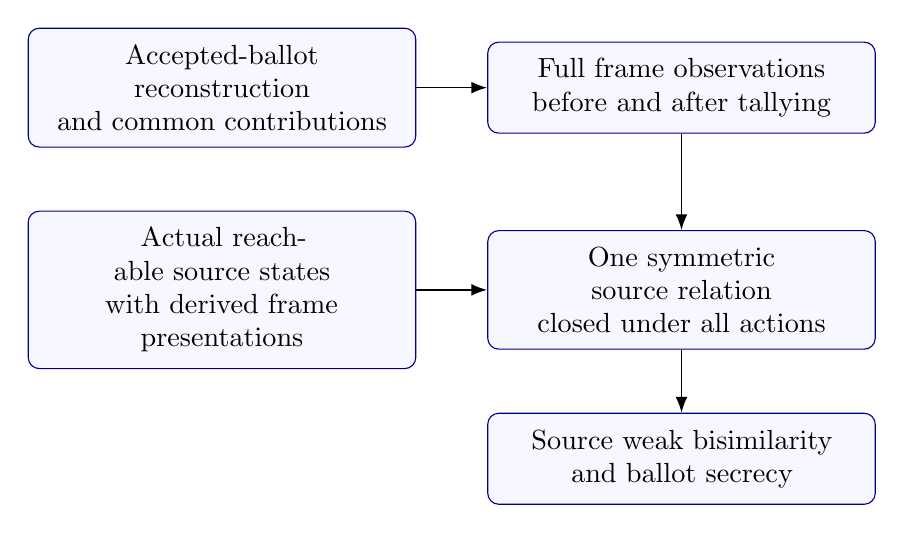
\begin{tikzpicture}[node distance=8mm and 9mm]
\node[box] (valid) {Accepted-ballot reconstruction\\and common contributions};
\node[box,right=of valid] (obs) {Full frame observations\\before and after tallying};
\node[box,below=of valid] (reach) {Actual reachable source states\\with derived frame presentations};
\node[box,right=of reach] (match) {One symmetric source relation\\closed under all actions};
\node[box,below=of match] (final) {Source weak bisimilarity\\and ballot secrecy};
\draw[arrow] (valid)--(obs);
\draw[arrow] (obs)--(match);
\draw[arrow] (reach)--(match);
\draw[arrow] (match)--(final);
\end{tikzpicture}
\end{center}
The diagram separates cryptographic observations from operational
correspondence. Both are required by the final theorem.

\subsection{What an accepted ballot contributes}
Proof validity yields semantic witnesses for the bit-valued ciphertext fields
and both kinds of proof. This is initially an existence result about terms;
it does not claim the attacker can recover honest secret nonces or votes.
The stronger accepted-ballot reconstruction uses publicness, the corrected
tail and the presence of both honest ballots on the board to reconstruct a
public constructor recipe for the submitted ballot.
\anchor{Symbolic/BallotValues}{proofValid_iff_values}
\anchor{Symbolic/GeneralAcceptedReconstruction}{Historical.General.accepted_ballot_constructor_recipe}

Here is the cross-world consequence used for accepted contributions. Write
$\varphi_s$ for the three-handle honest frame. Under name freshness, valid
$L,R$, a public recipe $r$ under $ns.\mathsf{restricted}$, and a recipe
board containing both honest ballot handles, acceptance of $r\varphi_0$
supplies one valid literal bit vector $b$ and public nonce recipes $\rho_j$:
\[
 \forall s\in\{0,1\}\ \forall j,\qquad
 \pi_j(r\varphi_s)\eqE\enc(K,\rho_j\varphi_s,b_j).
\]
This compresses the \code{SharedBallotData} record and its \code{Explains}
predicate. Shared objects are the bits and recipes; evaluated nonce values
need not be equal across worlds. Applying the result along accepted sequences
preserves the contribution alignment.
\anchor{Symbolic/AcceptedSequences}{Historical.General.initial_accepted_common_data}
\anchor{Symbolic/AcceptedSequences}{Historical.General.accepted_sequence_common_data}

\subsection{Acceptance and all transcript observations}
For public key, board and submission recipes, static equivalence transports
acceptance and rejection, also along board extensions. The honest-frame
theorem supplies the initial static-equivalence premise.
\anchor{Symbolic/AcceptedSequences}{Historical.General.initial_accepted_iff}
\anchor{Symbolic/AcceptedSequences}{Frame.StaticEq.acceptsSequence_iff}

Under $ns.\mathsf{Fresh}$, valid $L,R$, and world-0 phase reachability for
the chosen finite administration size, the completed observation result is
\[
 \mathsf{sourceView}(ns,0,L,R,p)\approx_s
 \mathsf{sourceView}(ns,1,L,R,p).
\]
This covers all public recipe equalities on the actual partial-decryption and
result expressions, including their tuple projections.
\anchor{Symbolic/SourceCapturedViews}{reachable_source_view_staticEq}

\subsection{From phases to arbitrary reachable source states}
Phases describe collection, checking and publication. Connecting them to
arbitrary structurally rearranged source states requires three further facts.

First, every finite original execution from $\W_s$ yields a reached phase,
name/channel and complete-handle bijections, a semantic phase connection, and
a structural presentation of the full frame. The inputs are the execution
and the final theorem's freshness conditions.
\anchor{Symbolic/SourceReachableFramePresentation}{source_reachable_frame_presentation}

Second, \code{SourceElectionRelation} carries both actual execution histories,
one common reached phase and coordinate system, semantic openings of both
states and both complete frame presentations. Initial membership is derived
from the scoped voters. Presentations are explicit because semantic realization
equality alone is insufficient (\S\ref{sec:controls}).
\anchor{Symbolic/SourceElectionRelation}{SourceElectionRelation}
\anchor{Symbolic/SourceElectionRelation}{SourceElectionRelation.initial}

Third, actual partner actions preserve this same relation:
\begin{center}\small
\begin{tabular}{@{}p{.22\linewidth}p{.66\linewidth}@{}}
\toprule
Action & Preserved obligation\\
\midrule
Internal & Match communication or either guard outcome in the actual partner.\\
Public input & Keep the literal channel and recipe and both successor presentations.\\
Fresh output & Keep the channel, every old handle, the fresh handle and full payload; derive the needed target name policy.\\
Structural change & Retain actual execution provenance and frame evidence.\\
Handle renaming & Use a common bijection preserving the complete exported domain.\\
\bottomrule
\end{tabular}
\end{center}
\anchor{Symbolic/SourceElectionRelation}{SourceElectionRelation.internal}
\anchor{Symbolic/SourceElectionRelation}{SourceElectionRelation.free}
\anchor{Symbolic/SourceElectionRelation}{SourceElectionRelation.bound}
\anchor{Symbolic/SourceElectionRelation}{SourceElectionRelation.structural}
\anchor{Symbolic/SourceElectionRelation}{SourceElectionRelation.reindex}

The final assembly packages symmetry, closedness, observations and successor
clauses as a weak labelled bisimulation. Matching uses one partner internal
step and zero surrounding silent steps for visible actions. Instantiation at
the actual initial source states proves the theorem in \S\ref{sec:theorem}.
\anchor{Symbolic/SourceBallotSecrecy}{source_reachable_weak_bisimulation}

\section{Counterexamples to proof shortcuts}\label{sec:controls}
These controls explain why some tempting simplifications would lose the target.
They are retained evidence; none is a missing premise in the final theorem.

\begin{counterexample}[Semantic equality does not give structural presentation]
Consider the source-local equation $\nu x.\{x/x\}$ and the empty process.
Under the realization semantics they have the same inhabited class: the
self-reference permits any local value. The original structural rules cannot
erase that self-reference to obtain the empty process.
\end{counterexample}
\anchor{Symbolic/SourceStructuralOpeningSPOT}{SourceStructuralOpeningSPOT.semantic_equality_is_insufficient}
\anchor{Symbolic/SourceStructuralOpeningSPOT}{SourceStructuralOpeningSPOT.insufficient_semantic_pair_is_inhabited}

Adding that unconstrained local to a complete live frame also fails to supply
a ground frame presentation, even though the semantic opening to the unpadded
state exists. This is a false general reconstruction claim, not a failed tactic.
The proof instead derives presentations for actual reachable election states,
using the necessary structural evidence.
\anchor{Symbolic/SourceBoundRigiditySPOT}{SourceBoundRigiditySPOT.changing_frame_values_or_policy_cannot_present_cycle}

\begin{counterexample}[An old frame policy need not describe the next output]
The process $\nu a.\overline c\langle a\rangle.0$ has an empty old frame,
which admits an empty restricted-name policy. After fresh-handle publication,
the frame records $x\mapsto a$ under the restriction of $a$. The old empty
policy cannot present the resulting frame. An appropriate new policy can.
\end{counterexample}
\anchor{Symbolic/SourceOutputFramePresentationSPOT}{SourceOutputFramePresentationSPOT.private_output_reconstructs_its_policy}
\anchor{Symbolic/SourceOutputFramePresentationSPOT}{SourceOutputFramePresentationSPOT.reconstructed_policy_cannot_be_the_old_empty_policy}

The fixture uses base name 40 and public channel 0. This is a failure of an
insufficient policy invariant. Fresh-output reconstruction derives the target
policy from the whole live process, rather than freezing it to the old frame's
minimal policy.

\begin{counterexample}[Static equivalence alone misses behavior]
An output-capable state and a stopped state have equivalent current frames
but are not weakly labelled bisimilar. The stopped state cannot silently
manufacture the output channel. A separate control rules out declaring a
missing exported handle domain equivalent to a complete one.
\end{counterexample}
\anchor{Symbolic/SourceBallotSecrecySPOT}{SourceBallotSecrecySPOT.static_equivalence_does_not_prove_weak_bisimilarity}
\anchor{Symbolic/SourceBallotSecrecySPOT}{SourceBallotSecrecySPOT.missing_domain_is_not_weakly_bisimilar}

At the historical source level, a replay input and subsequent rejection are
matched by the final relation. The theorem is also instantiated for every
finite additional-input count. These complement the finite model's independent
valid-ballot and nonconstant-tally controls.
\anchor{Symbolic/SourceBallotSecrecySPOT}{SourceBallotSecrecySPOT.actual_replay_rejection_is_weakly_matched}
\anchor{Symbolic/SourceBallotSecrecySPOT}{SourceBallotSecrecySPOT.arbitrary_administration_secrecy}

\section{Concrete ballot proofs}\label{sec:concrete}
The \href{../../ExplainableCrypto/Helios/Computational/README.md}{computational development} uses
VCVio for probability semantics and cryptographic algorithms, with Lean/Mathlib
4.33.1 for the shared formal development. The exact vulnerable construction is Smyth's
at-most-one variant with abstention and component weeding~\cite{smyth}.
The \href{../research/helios-computational-model.md}{concrete model} records its
public transcript and construction boundaries. The computational secrecy
statement is in Section~\ref{sec:computational-final}.

Write ElGamal as $E_h(r,m)=(g^r,g^m h^r)$ in a prime-order group. Each branch
$i\in\{0,1\}$ of a ballot proof contains $(A_i,B_i,c_i,s_i)$ and verifies
\[
 g^{s_i}=A_i a^{c_i},\qquad
 h^{s_i}=B_i(b/g^i)^{c_i},\qquad
 c_0+c_1=H(A_0,B_0,A_1,B_1).
\]
The last equation is shared by both branches. The hash input here contains
only commitments. Honest zero/one proof constructors satisfy these equations
for every hash function; the algebraic lemmas allow arbitrary scalar values.
The encryption body is identified with VCVio's algorithm. A separate historical
sampler assigns probability $1/(|F|-1)$ to each nonzero scalar. With injective
generator exponentiation, honest encryption never produces $(1,1)$.
\companchor{BallotProof}{proveZero_valid}
\companchor{BallotProof}{proveOne_valid}
\companchor{Sampling}{sampleNonzero_probability}
\companchor{Sampling}{honestEncrypt_ne_neutral}

\begin{theorem}[Neutral-ciphertext proof]
For any scalars $e,z,w$, set
\[
 \begin{gathered}
 (A_0,B_0)=(g^w,h^w),\qquad (A_1,B_1)=(g^z,h^z g^e),\\
 c_1=e,\qquad c_0=H(A_0,B_0,A_1,B_1)-e,
 \end{gathered}
\]
and $s_0=w,s_1=z$. This proof verifies for $(a,b)=(1,1)$ for every $H$,
without a secret key.
\end{theorem}
\companchor{BallotProof}{neutralProof_valid}

Replacing an earlier valid ballot's components by their product in the first slot
and $(1,1)$ in all other slots preserves proof validity: copy its aggregate
proof into the first and aggregate proof positions, and use neutral proofs
elsewhere. For at least two components, this ballot passes weeding exactly
when its aggregate and $(1,1)$ each avoid every earlier board component.
This characterizes freshness on arbitrary boards; Section~\ref{sec:concrete-collisions} gives a
sufficient nonce condition and a probability bound for honest ballots.
\companchor{ProofReuse}{proofReuse_valid}
\companchor{ProofReuse}{proofReuse_fresh_iff}

Independent fixtures use $p=23,q=11,g=2,h=8$ and a fixed hash challenge 5.
Lean checks the constructors' encoded group values and the verification
equations; changing a response is rejected. These fixtures test arithmetic,
not cryptographic hardness or SHA-256. Section~\ref{sec:concrete-game} connects
the attack to probability. The concrete repair is checked in Section~\ref{sec:concrete-repair};
Section~\ref{sec:computational-final} states secrecy under explicit implementation assumptions.
\companchor{Controls}{Controls.neutral_constructor_matches}
\companchor{Controls}{Controls.changed_response_rejected}

\section{Honest ballots and nonce collisions}\label{sec:concrete-collisions}
The checked two-component honest ballot for $v\in\{0,1\}$ is
$(E_h(r_0,v),E_h(r_1,0))$. Its component and aggregate proofs use the concrete
zero/one constructors; its aggregate encrypts $v$ with nonce $r_0+r_1$.
All proofs validate for arbitrary proof coins and every commitment hash.
This covers abstention and the first candidate, as needed for the intended
swapped-world attack experiment.
\companchor{HonestBallot}{honestBallot_valid}

Let the second honest ballot use nonces $s_0,s_1$. Suppose all four nonces
are nonzero and generator exponentiation is injective. Define
\[
 \mathsf{Good}(r,s)\iff
   (\forall i,j\in\{0,1\},\ r_i\ne s_j)
   \land (\forall j\in\{0,1\},\ r_0+r_1\ne s_j).
\]
Under this condition, the second honest ballot passes component weeding
against the first, and the proof-reuse ballot from the first passes weeding
against both. This holds for either honest vote and arbitrary proof coins.
The conditions are derived from equality of actual ciphertext components.
They do not assume a symbolic correspondence.
\companchor{HonestBallot}{honestBallot_fresh}
\companchor{HonestBallot}{proofReuse_honest_fresh}

For a finite field $F$ and fixed $r_0,r_1$, draw $s_0,s_1$ independently and
uniformly from $F\setminus\{0\}$. Then
\[
 \Pr\bigl[\exists j\in\{0,1\},\ s_j\in\{r_0,r_1,r_0+r_1\}\bigr]
 \le \frac{6}{|F|-1}.
\]
Lean derives this union bound from VCVio's probability semantics and the
nonzero sampler. Repeated forbidden values only loosen the bound.
\companchor{CollisionProbability}{pairCollision_probability_le}

\paragraph{Retained counterexample.}
If the second nonces agree, both honest ballots contain the same zero
component. Their proofs validate, but the second ballot fails weeding.
Thus unconditional acceptance of independently sampled honest ballots is
false. The counterexample is a general checked implication, not a failed
search for an acceptance proof.
\companchor{HonestBallot}{coincident_honest_ballots_not_fresh}

The full honest sampler extends this bound through both nonce pairs and all
proof randomness. It does not resample on collisions or discard rejected runs.
\companchor{HonestSampling}{drawHonestPair_collision_le}

\section{The public probabilistic attack}\label{sec:concrete-game}
The implemented experiment has two candidates, two honest voters, one dishonest
voter and one honest trustee. The challenger samples a uniform hidden bit $v$;
honest ballots encode $v$ and $1-v$ in the first candidate. Trustee secrets,
proof coins and encryption nonces use the historical nonzero sampler.

The attacker sees the parameters, key proof, fingerprint, honest decisions and
accepted identified ballots. It submits the first ballot's aggregate followed
by a neutral ciphertext, with the reused and neutral proofs above. Submission
checks are actual proof verification and component weeding. Rejection retains
the board and tallying continues. The final public message includes the
submission decision, accepted board, encrypted tallies, decryption shares and
proofs, and bounded tally decoding (including decoding failure).
\companchor{Board}{submit_rejected_preserves_board}
\companchor{AttackGame}{executeAttack_key_proof_valid}
\companchor{AttackGame}{executeAttack_decryption_proofs_valid}

On $\mathsf{Good}$, all three ballots are accepted and public decryption of the
first tally yields $g^{1+v}$. The attacker returns true exactly when this group
element equals $g^2$. It uses neither the secret key nor honest coins.
\companchor{AttackGame}{executeAttack_on_good}

\begin{theorem}[Concrete proof-reuse success]
Let $F$ be a finite field and $G$ an $F$-module with decidable equality. Suppose
$r\mapsto r\mathbin{\bullet}g$ is injective. For every choice of the typed ballot,
key-proof, decryption-proof and fingerprint hashes, the public proof-reuse
attacker in \code{ballotSecrecyGame} satisfies
\[
 \Pr[\mathsf{guess}=v]\ \ge\ \max\left(0,\ 1-\frac{6}{|F|-1}\right).
\]
\end{theorem}
The Lean statement uses truncated subtraction in $\mathrm{ENNReal}$. The
proof bounds all bad-event executions; freshness is derived, not assumed.
The bound exceeds one half when $|F|-1>12$.
\companchor{BallotSecrecyGame}{instantiated_attack_game}
\companchor{BallotSecrecyGame}{ballotSecrecyGame_proofReuse_success}

Independent modulo-23 fixtures check the published trustee proofs, decoded
tallies 1 and 2, invalid-proof rejection, retained-board tallying after honest
rejection, and a fresh abstention with no copying effect.
\companchor{ExecutionControls}{ExecutionControls.rejection_retains_board_and_tally_continues}
\companchor{ExecutionControls}{ExecutionControls.fresh_abstention_has_no_copying_effect}

This is a cast-only attack witness with typed subgroup inputs and a fixed
eligible-identity schedule. Byte parsing, non-subgroup inputs, an authentication
implementation and a security-parameter/PPT backend are outside the checked
game. The optional audit-and-discard path is unused. The concrete repair follows
next; Section~\ref{sec:computational-final} gives its scoped secrecy theorem.

\section{Concrete repair and honest correctness}\label{sec:concrete-repair}
The selected repair follows Bernhard--Pereira--Warinschi~\cite{bpw}: hash the
statement as well as commitments, and include implicit aggregate ciphertexts in
weeding. For a ballot proof, the challenge now hashes $(g,h,(a,b))$ and the four
commitments. Key and decryption proofs also hash their statements. The branch
equations and homomorphic encryption remain the same.
\companchor{StrongBallot}{strongHonestBallot_valid}

For ballot $b$, let $C(b)$ contain its components and implicit aggregate.
Expanded weeding requires
\[
  \forall b'\in\mathsf{board},\ \forall c\in C(b),\ \forall c'\in C(b'),\quad c\ne c'.
\]
A submitted first component equal to an earlier aggregate fails this test.
This is a check on the actual group ciphertexts, independent of hash security.
\companchor{StrongBallot}{copied_aggregate_not_expanded_fresh}

\begin{theorem}[Known attack rejected]
In the repaired three-voter execution, Smyth's copied-aggregate submission is
rejected as a reused ciphertext for every choice of honest coins and typed
hashes. The previously accepted board is retained and tallying continues.
Under the finite-field sampler, the rejection probability is one.
\end{theorem}
\companchor{RepairedExecution}{executeRepairedAttack_rejected}
\companchor{RepairedBoard}{repairedSubmit_rejected_preserves_board}
\companchor{RepairedGame}{repairedAttackWorld_rejection_probability}

\paragraph{Honest correctness and collisions.}
Honest strong proofs validate for every typed hash. If the two honest nonce
sets $\{r_0,r_1,r_0+r_1\}$ and $\{s_0,s_1,s_0+s_1\}$ are disjoint and generator
exponentiation is injective, both ballots are accepted. Their decrypted group
tally is $(g,1_G)$ in either swapped world. For independently sampled nonzero
coins, accidental rejection has probability at most $9/(|F|-1)$. The extra
three terms cover the second aggregate nonce; no collision runs are removed.
\companchor{RepairedBoard}{repairedHonestPair_decrypts}
\companchor{RepairedSampling}{repairedHonestPair_rejection_le}

\paragraph{Both repair components matter.}
With weak hashes, rerandomizing $(a,b)$ to $(ag^u,bh^u)$ and changing each
response to $s_i+c_i u$ preserves verification for every hash. Conversely,
strong statement hashes alone still validate Smyth's copied aggregate: its
ciphertext statement is unchanged. Independent controls retain both failures
and check accepted honest ballots, literal trustee transcripts and nonconstant
tallies under the full repair.
\companchor{WeakProofMalleability}{Proof01.rerandomize_valid}
\companchor{StrongBallot}{strongProofReuse_valid}
\companchor{RepairControls}{RepairControls.honest_valid_attack_rejected_and_tally_preserved}

The implemented instance retains the historical nonzero sampler and cast-only
scope. BPW uses full-field sampling and a different simulated-tally privacy
game. Its published theorem is not an imported reduction. Adaptive extraction
for the actual disjunctive proof and the finite DDH reduction are checked;
Section~\ref{sec:computational-final} gives the final theorem with external efficiency.

\section{Computational game and ballot secrecy}\label{sec:computational-final}
Fix a security parameter $n$, prime scalar field $F_n=\mathbb Z/q(n)\mathbb Z$
and group $G_n$ with distinguished element $g_n$. We use additive group notation, so the
public key is $x\mathbin{\bullet}g_n$. The notation dictionary from
Section~\ref{sec:concrete} is
\[
  g^r \longleftrightarrow r\mathbin{\bullet}g_n,
  \qquad uv \longleftrightarrow u+v, \qquad 1_G \longleftrightarrow 0_G.
\]
Thus the same ElGamal ciphertext $(g^r,g^m h^r)$ is written
$(r\mathbin{\bullet}g_n,\,m\mathbin{\bullet}g_n+r\mathbin{\bullet}h)$,
with $h=x\mathbin{\bullet}g_n$; only the group notation changes.
The election has two candidates, honest
voters 0 and 1, attacker-controlled voter 2, and one honest trustee. The secret
bit selects which honest voter casts the first-candidate vote and which abstains;
the second candidate coordinate is always zero. This section uses the
statement-bound hashes and component/aggregate freshness repair of
Section~\ref{sec:concrete-repair}.

\begin{figure}[!ht]
\centering
\fbox{\begin{minipage}{.93\linewidth}
\textbf{Guessing experiment $\mathsf{BS}_A(n)$}
\begin{enumerate}[leftmargin=1.6em,itemsep=3pt]
\item Start with an empty shared random-oracle cache $H$.
Run $i\leftarrow A_{\rm prepare}(n)$; its queries update $H$.
\item Draw a uniform bit $b$. Draw the trustee secret, key-proof nonce,
two decryption-proof nonces and both honest ballots' coins using the specified
nonzero samplers. No collision is conditioned away.
\item Construct the key proof and public parameters. Construct and submit
honest ballots for choices $b$ and $\neg b$, in voter order, using repaired
validation. Let $v$ contain the parameters, fingerprint, both submission
decisions and retained honest board.
\item Run $(B,s)\leftarrow A_{\rm cast}(n,i,v)$.
Validate $B$ as voter 2 against the retained board. Rejecting $B$ preserves that
board; either decision proceeds to tallying.
\item Aggregate the retained board, produce both trustee shares and their
proofs, and perform bounded decoding. Form $w$ from $v$, submitted ballot $B$,
the decision, final board, encrypted tally, shares, proofs and optional decoded
results, including decoding failure.
\item Run $\widehat b\leftarrow A_{\rm guess}(n,i,s,w)$.
Return $[\widehat b=b]$.
\end{enumerate}
All proof generation, validation and attacker callbacks share $H$. Hash keys
are tagged by proof type and contain the full statement and commitment.
A repeated key reuses its answer; a new key receives a uniform field element.
Attacker callbacks also have the specified finite-uniform sampling interface.
\end{minipage}}
\caption{The fixed computational ballot-secrecy game. The cache and private
states are not added to the public transcript; the attacker retains its own
query answers. This is a compression of the original game, before query clocking.}
\label{fig:computational-game}
\end{figure}
\companchor{ElectionOracle}{ElectionOracle.preparedGame}
\companchor{ElectionOracle}{ElectionOracle.game}
\companchor{ElectionOracle}{ElectionOracle.world}
\companchor{ElectionOracle}{ElectionOracle.prefixWithCoins}
\companchor{ElectionOracle}{ElectionOracle.finishWithCoins}
\companchor{ElectionOracle}{ElectionOracle.run_ask}

\begin{definition}[Ballot-secrecy bias]
For the experiment in Figure~\ref{fig:computational-game}, define
\[
 \beta_A(n)=\left|\Pr[\mathsf{BS}_A(n)=1]-\frac12\right|.
\]
The probability includes preparation, the secret bit, protocol and attacker
randomness, and the shared random oracle. A nonnegative function $f$ is
negligible when $n^d f(n)\to0$ for every fixed $d\in\mathbb N$.
\end{definition}
\companchor{ElectionSecurityFamily}{ElectionSecurityFamily.Family.bias}

The game exposes complete retained-board and rejection behavior. It does not
assert privacy for other observation schedules, corrupt trustees, more voters,
or a larger challenge family. The conditions below describe exactly the
encoded attacker interface covered by the theorem.

\subsection{Parameters and attacker resources}\label{sec:family-resources}
Write $F_n=\mathbb Z/q(n)\mathbb Z$. A value $A$ of
\code{ElectionSecurityFamily.Family} supplies the following data and properties.
All polynomials have natural coefficients. The resource conditions concern the
\emph{original} callbacks, before the derived query clocks are applied.

\begin{longtable}{@{}>{\raggedright\arraybackslash}p{.28\linewidth}>{\raggedright\arraybackslash}p{.64\linewidth}@{}}
\textbf{Data or condition}&\textbf{Required property}\\\hline
Scalar and group family&For each $n$, $q(n)$ is prime; $G_n$ is an additive
commutative group and an $F_n$-module, with decidable equality.\\
Group representation&An injective encoding of every $G_n$ element into bits,
with one polynomial upper bound $R(n)$ on its length.\\
Scalar width&The binary width of $q(n)$ is at most a polynomial $Q(n)$.
A public scalar is encoded by the bits of its canonical representative.\\
Fingerprint&Its output has binary width at most a polynomial $F(n)$ for every
parameter record whose candidate and eligible lists are exactly $[0,1]$ and
$[0,1,2]$. All typed group/scalar assignments to such records are covered.\\
Generator&The map $r\mapsto r\mathbin{\bullet} A.\code{generator}(n)$ is injective.\\
Private state&Arbitrary families \code{Init} and \code{Saved}, each with an
injective bit encoding. Private sizes below are actual encoding lengths.\\
Original source&The preparation computation and the preparation-dependent
cast/guess callbacks, with the existing typed oracle interface.\\
Preparation&At most $P(n)$ queries; every output in its source support has
encoded \code{Init} length at most $I(n)$.\\
Casting&At most $C(n+|i|+|\operatorname{encPrefix}(v)|)$ queries for every
initial state $i$ and public prefix $v$. Every cast output has encoded saved
state length at most $S(n+|i|+|\operatorname{encPrefix}(v)|)$.\\
Guessing&At most $J(n+|i|+|s|+|\operatorname{encResult}(w)|)$ queries for every
initial state $i$, saved state $s$, and public result $w$.\\\hline
\end{longtable}

Here $P,I,C,S,J$ are the fields \code{prepareCost}, \code{initGrowth},
\code{castCost}, \code{savedGrowth}, and \code{guessCost}, respectively.
Query bounds and source support range over \emph{all well-typed replies},
including inconsistent answers to repeated hash queries. Pure output growth is
bounded separately: a query count does not bound local work or private storage.
These are resource properties, not a supplied correspondence with the game.
\companchor{ElectionSecurityFamily}{ElectionSecurityFamily.Family}

\paragraph{Derived representation and coverage.}
The public lengths above are literal encodings of every field of the existing
\code{PublicPrefix} and \code{PublicResult}. Generic injectivity preserves
observations; specialization to the established prime codecs is exact. The
checked serialization bounds include all nested framing. In particular, let
$L=R+Q+F+1$, $B_0=100(L+1)$ and $B_1=B_0+1000(L+1)$. Reached structural widths
are bounded by $B_0(n)$ and $B_1(n)$, and reached encoded lengths by
$10^8B_0(n)$ and $10^{10}B_1(n)$. The fixed constants are conservative proof
bounds, not measured costs. The source proof retains rejected submissions:
there are at most two board entries before casting and three afterward, and
any successful decoded value is at most three.
\companchor{ElectionPublicEncoding}{ElectionPublicEncoding.prefix_injective}
\companchor{ElectionPublicEncoding}{ElectionPublicEncoding.result_injective}
\companchor{ElectionPublicEncoding}{ElectionPublicEncoding.prime_prefix_eq}
\companchor{ElectionPublicEncoding}{ElectionPublicEncoding.prime_result_eq}
\companchor{ElectionPublicEncoding}{ElectionPublicEncoding.prefix_length_le}
\companchor{ElectionPublicEncoding}{ElectionPublicEncoding.result_length_le}

Polynomial composition therefore gives
\[
\begin{aligned}
V&=X+I+10^8B_0,& C_*&=C\circ V,&S_*&=S\circ V,\\
Z&=X+I+S_*+10^{10}B_1,&J_*&=J\circ Z.
\end{aligned}
\]
The normalized family $D=A.\code{prepared}$ keeps preparation unchanged and
clocks casting and guessing at $C_*(n)$ and $J_*(n)$. Its saved type is
\code{Option Saved}. A cast timeout returns an explicit zero ballot and absent
state; a guess timeout or absent saved state returns false.
No private default or acceptance of this fallback is assumed. The reached-input
bounds prove clock transparency, including the original private states and
public results. Thus \code{coverage} is equality of complete oracle computations;
\code{run_coverage} retains the full output and final shared cache from every
starting cache. \code{bias_eq} identifies the original game's bias.
\companchor{QueryClock}{QueryClock.eq_of_total_bound}
\companchor{ElectionSecurityFamily}{ElectionSecurityFamily.Family.coverage}
\companchor{ElectionSecurityFamily}{ElectionSecurityFamily.Family.run_coverage}
\companchor{ElectionSecurityFamily}{ElectionSecurityFamily.Family.bias_eq}

\subsection{Accuracy and the secrecy theorem}\label{sec:accuracy}
The main DDH reduction uses repeated extraction attempts. For a fixed
\emph{accuracy degree} $k\in\mathbb N$, its accuracy request is
\[
 a_k(n)=(n+1)^{k+1}.
\]
The finite reduction has residual slack $2/a_k(n)$ plus terms that are negligible
under the stated assumptions. For each fixed $k$, the number of extraction
attempts is polynomial in $n$; increasing $k$ changes that polynomial and may
change the realizing machine. The assumption is $\forall k\,\exists M_k,P_k$,
not a single bound jointly polynomial in $n$ and varying $k$.
The inequality $n^k\,2/a_k(n)\le 2/(n+1)$ explains why a separate reduction
for every fixed accuracy degree suffices to prove negligibility. One fixed
inverse-polynomial slack would not suffice.
\companchor{ElectionSecrecyPrototype}{ElectionSecrecyPrototype.accuracy}
\companchor{ElectionSecrecyPrototype}{ElectionSecrecyPrototype.negligible_of_polynomial_accuracy}

Write $\mathsf{Eff}_{\rm enc}(D)$ when one finite uniform fair-coin machine
realizes the exact output distribution of the family $D$ and halts within a
fixed polynomial in $n$ on every encoded challenge and every coin path.
Its precise machine convention and relation to ordinary PPT are given below.
Let $D^{\rm main}_{A,k}$ and $D^{\rm reject}_A$ denote the exact main and
rejection distinguishers constructed from the normalized family $A.\code{prepared}$.
For a distinguisher $D$, define its DDH advantage by
\[
 \Delta_D(n)=\left|
 \Pr[D_n(g_n,xg_n,yg_n,(xy)g_n)=1]
 -\Pr[D_n(g_n,xg_n,yg_n,zg_n)=1]\right|,
 \qquad x,y,z\leftarrow F_n.
\]
Scalar multiplication abbreviates $x\mathbin{\bullet}g_n$, and each challenge
uses the same fixed injective group encoding as the election family.
\companchor{ElectionSecrecyFairBits}{ElectionSecrecyFairBits.main}
\companchor{ElectionSecrecyFairBits}{ElectionSecrecyFairBits.reject}
\companchor{ReductionEfficiency}{ReductionEfficiency.Efficient}
\companchor{ReductionEfficiency}{ReductionEfficiency.DDHAssumption}

\noindent\begin{minipage}{\linewidth}
\begin{theorem}[Computational ballot secrecy; compressed mathematical statement]
For every parameter and attacker family $A$ satisfying all conditions in
Section~\ref{sec:family-resources}, let $D=A.\code{prepared}$ be the
normalization defined above. Suppose:
\begin{enumerate}
\item $1/(q(n)-1)$ is negligible;
\item for every fixed $k$, $\mathsf{Eff}_{\rm enc}(D^{\rm main}_{A,k})$;
\item $\mathsf{Eff}_{\rm enc}(D^{\rm reject}_A)$;
\item for every distinguisher family $E$ with $\mathsf{Eff}_{\rm enc}(E)$,
      its DDH advantage $\Delta_E$ is negligible.
\end{enumerate}
Then the original game's ballot-secrecy bias is negligible:
\[
             \forall d\in\mathbb N,\qquad
             \lim_{n\to\infty} n^d\,
             \left|\Pr[\mathsf{BS}_A(n)=1]-\tfrac12\right|=0.
\]
\end{theorem}
\end{minipage}

\companchor{ElectionSecurityFamily}{ElectionSecurityFamily.Family.ballot_secrecy}
Hypotheses 2 and 3 are the usual proof step that the constructed reductions run
in polynomial time. They are explicit here because the development defines a
machine-cost model but does not prove polynomial-time realizations of these two
complete reductions. Section~\ref{sec:standard-ddh} gives the external efficiency
arguments and relates the chosen machine convention to conventional PPT.

The first assumption is the Lean quantity \code{noncePointBound} for the prime
field, namely $1/(q(n)-1)$. It is equivalent here to negligible $1/q(n)$:
for primes $q\ge2$, $1/q\le1/(q-1)\le2/q$. The theorem retains both explicit
implementation hypotheses; it does not derive them from query counts. The full
Lean interface appears in Appendix~\ref{sec:lean-interface}.


\subsection{How the computational reduction proves secrecy}\label{sec:computational-proof}
The checked reduction retains preparation, both public interaction points,
rejection decisions and the public transcript fields. It first replaces the honest
proofs with programmed random-oracle simulations, accounting for the difference
introduced by the historical nonzero sampling rule. Repeated extraction obtains
witnesses for accepted attacker contributions except on a bounded failure event,
while retaining the original execution and saved state. An extracted finisher produces the public result
without access to the DDH challenge's secret scalar. A separate distinguisher
accounts for observable honest rejection.

In the mathematical random-DDH comparison hybrid, which has a secret-key
argument, a uniform mask can be translated by the honest
vote without changing its distribution. The complete unscored public
continuation is thereby independent of the secret bit, so the guess succeeds
with probability $1/2$. This is a claim about the full continuation, not just
its tally. The extraction and simulation comparisons connect this hybrid to
the actual game.
\companchor{ElectionDDHRandomSource}{ElectionDDHSource.completed_random_win}
\companchor{ElectionSecrecyPrototype}{ElectionSecrecyPrototype.prepared_negligible_of_ddh}

For the normalized family, write $p(n)=P(n)$ and $c(n)=C_*(n)$.
For every fixed $k$, the checked ideal-sampling reduction gives, for all
sufficiently large $n$,
\[
\begin{split}
 \beta_A(n)\ \le\ &\frac{18}{q(n)-1}
 +\frac{3(11p(n)+2c(n)+131)}{q(n)}
 +\frac{2}{a_k(n)}\\
 &+\Delta^{\rm ideal}_{{\rm main},k}(n)
 +\Delta^{\rm ideal}_{\rm reject}(n).
\end{split}
\]
Here the two ideal advantages use the exact finite-uniform samplers before
fair-bit replacement. The field-size side condition of the finite bound holds
eventually because $p,c,a_k$ are polynomial and the inverse field size is
negligible. Fair-bit transport adds negligible sampling losses and replaces
these two advantages by those of the exact machine-realized reductions.
DDH makes the latter negligible; varying the fixed accuracy degree as above
removes the remaining inverse-polynomial slack. Finally, the checked equality
of the clocked and original games identifies their biases.
\companchor{ElectionSecrecyPrototype}{ElectionSecrecyPrototype.accuracy_admissible}
\companchor{ElectionSecrecyFairBits}{ElectionSecrecyFairBits.prepared_negligible_of_fair_bits}
\companchor{ElectionSecurityFamily}{ElectionSecurityFamily.Family.bias_eq}


\subsection*{Correspondence with the four Lean hypotheses}
Beyond $A$ and its family conditions, \code{Family.ballot_secrecy} has exactly
these four hypotheses and concludes negligible original prepared-game bias.

\begin{longtable}{@{}>{\raggedright\arraybackslash}p{.28\linewidth}>{\raggedright\arraybackslash}p{.64\linewidth}@{}}
\textbf{Hypothesis}&\textbf{Meaning}\\\hline
\code{hsize}&The original \code{noncePointBound} of $F_n$ is negligible.
This lower-growth requirement on field size is separate from encoded-width
upper bounds.\\
\code{hmain}&\code{MainReductionEfficient} for $D$ and the same group
representation: for every fixed accuracy degree $k$, one uniform finite program
realizes the exact normalized main reduction within a polynomial in $n$.\\
\code{hreject}&\code{RejectionReductionEfficient} for that exact $D$ and
representation.\\
\code{hddh}&DDH against the explicitly defined uniform machine class under
the same representation and generator family.\\\hline
\end{longtable}

A realization contains finite coin-only code, a polynomial clock, halting with
an actual Boolean output on every coin path, and exact output-distribution
agreement on every challenge quadruple. Its input is unary $n$ followed by four
separately framed group words. Before a coin command the answer tape must be
blank, excluding an uncharged bulk erasure. There are no arithmetic, callback,
hash or storage oracles in this machine. Each fixed $k$ may choose its own code
and polynomial; no bound jointly polynomial in varying $k$ is asserted.
The constant-false control inhabits the generic realization predicate, not the
exact reductions or the combined cryptographic hypotheses.
\companchor{ReductionEfficiency}{ReductionEfficiency.Realization}
\companchor{ReductionEfficiency}{ReductionEfficiency.MainReductionEfficient}
\companchor{ReductionEfficiency}{ReductionEfficiency.RejectionReductionEfficient}
\companchor{ElectionSecurityFamily}{ElectionSecurityFamily.Family.ballot_secrecy}

\subsection{Relation to conventional PPT and standard DDH}\label{sec:standard-ddh}
\textbf{External mathematical argument.}
Every family satisfying $\mathsf{Eff}_{\rm enc}$ has an implementation by a
conventional strict probabilistic polynomial-time Turing machine on the same
encoded challenges. Only this inclusion is needed; no equivalence of machine
classes is claimed as a Lean theorem.

To see the inclusion, fix a realization. Its finite labels and three head cells,
each holding a Boolean or blank, determine a finite transition table. A local
command performs only a fixed number of head moves or cell writes. Hash commands
are excluded. On every valid run, the answer tape is blank before a fair-coin
command, so that command can be implemented by a coin flip and one local write,
without bulk erasure. Thus a conventional multitape probabilistic machine
simulates the steps with bounded overhead; a single-tape simulation has
polynomial overhead. This is a simulation of the defined tape operations, not a
claim about the runtime of evaluating the Lean interpreter.

The realization guarantees halting within a polynomial $T(n)$ only on valid
challenge encodings. To obtain a strict machine on arbitrary bit strings, parse
the unary parameter and field framing, reject malformed framing, and enforce
the known polynomial clock while simulating. No group-membership test is needed:
a string with well-formed framing but invalid group words can time out and return
a fixed bit. Parsing costs polynomial time in input length $N$, and $n\le N$.
Clock construction and simulation therefore cost polynomial time in $N$ on all
inputs. On valid challenges the clock does not alter the output distribution. The
checked bound $N\le n+8R(n)+5$, where $R$ bounds group encoding width, also
makes this runtime polynomial in the security parameter on those challenges.
\companchor{ReductionEfficiency}{ReductionEfficiency.inputWord}
\companchor{ReductionEfficiency}{ReductionEfficiency.inputWord_length}
\companchor{ReductionEfficiency}{ReductionEfficiency.Realization}

Consequently, \emph{standard DDH against conventional strict PPT machines for
these same encodings and challenge distributions implies the DDH hypothesis used
by the Lean theorem}. Challenges lie in the order-$q(n)$ subgroup generated by
$g_n$; the formal parameter conditions do not require $g_n$ to generate all of
$G_n$. A DDH assumption stated with a different representation would additionally
need an efficient translation preserving the distribution. Injectivity and
polynomial encoded width alone do not supply that translation. This external
inclusion establishes neither of the exact reduction-efficiency hypotheses;
those are the separate implementation claims discussed next.


\paragraph{External claim E1: attacker membership.}
Use uniform, explicitly polynomial-clocked strict oracle-PPT callback
implementations with effective canonical representations. Charge writing query
indices, processing replies, copying suspended configurations and serializing
returned private state. A strict time polynomial in unary $n$ plus actual
encoded input length bounds both query count and serialized private output.
Enlarging constants and coefficients gives $P,I,C,S,J$. Hash replies have the
stated scalar width. A uniform-range index must be written by the attacker;
its reply has at most that index's polynomial bit width. Effective scalar/group
operations and fingerprint evaluation obey the fixed parameter policy.
These facts supply local family resources; the Lean coverage proof, rather than
an external game-correspondence hypothesis, derives transparency of the query
clocks on reached inputs.

The clock convention applies to every typed reply sequence. A guarantee only
against consistent hash functions is not the same premise. The independent
finite control asks the same key twice and makes a third request only on
unequal answers: every fixed singleton-key handler gives two requests, but its
complete tree needs three. This refutes transfer of the same finite bound,
not a general asymptotic claim. Given a known strict polynomial bound on all
consistent executions, an external time-clock normal form preserves their oracle
interactions, private outputs and output law, and stops other reply paths. That normalization is an
external argument; \code{Family.coverage} does not itself establish it for an
arbitrary pre-existing unclocked source callback. The stated membership claim
uses the explicitly clocked model. Expected-time-only attackers are outside
this argument.
\companchor{ElectionCoverageControls}{ElectionCoverageControls.fixed_hash_two_requests}
\companchor{ElectionCoverageControls}{ElectionCoverageControls.consistent_bound_not_syntactic_bound}

\paragraph{External claim E2: exact normalized reduction efficiency.}
Fix $k$ and uniform correct implementations of the actual primitives and
callbacks, including all altered replay response paths. Their local runtime,
full configuration widths, scalar/group widths, query indices and stored
responses have polynomial envelopes. The actual normalized budgets are
$p=P(n)$ and $c=C_*(n)$, evaluations of fixed polynomials; thus the repetition
count is uniformly computable, not merely bounded by a computable function.
The checked query bounds give
\[
M=4P(n)+4C_*(n)+78,\qquad
R_k=3456\bigl(P(n)+C_*(n)+10\bigr)^3(n+1)^{4(k+1)}.
\]
Rejection uses at most $M$ queries and main at most
$(1+3R_k)M+4+4J_*(n)$. The rejection prefix includes the actual cast.
\companchor{ElectionDDHRejection}{ElectionDDHSource.honestReject_total_bound}
\companchor{ElectionDDHReduction}{ElectionDDHSource.ballotSecrecy_prime_cost}

Implement dictionaries and logs as finite lists. The representation invariant
identifies auxiliary, live and programmed lookups with their source caches,
retains the sticky flag and ordered history, and identifies callback snapshots
and replay tapes with their original configurations and answers. A hit returns
the stored value without sampling; a miss performs the source draw and update.
Programming follows the actual occupied-key rule and keeps the live cache
separate. Induction over these operations preserves the invariant. The checked
finite-cache laws and auxiliary-source interpretation identify the operations;
they do not by themselves compile this whole implementation.
\companchor{BallotFiniteCache}{runBallotFiniteCache_eq}
\companchor{BallotFiniteCache}{runBallotFiniteCache_length_le}
\companchor{ElectionReplaySource}{ElectionReplaySource.lower_run}

Each replay attempt starts from the same recorded original path. Copying a
snapshot or reconstructing it with recorded answers has polynomial cost.
A failed residual's enlarged state is not passed to the next attempt. The final
continuation uses the original retained state/cache. Source bad, rejection,
extraction-failure and normalized-timeout branches remain executed. Using the
same fresh fair bits for corresponding draws preserves the exact output law,
not only a support condition or a successful-run projection.
\companchor{BallotReplayRepeat}{ballotJointReplayRepeatAtPath}
\companchor{ElectionDDHPrefixRepeat}{ElectionDDHSource.prefix_repeated_original}
\companchor{ElectionDDHExtractedFinish}{ElectionDDHSource.extractedGame}

The bounded sampler reads the source-prescribed number of bits and computes
modulo the requested range, with polynomial binary arithmetic. Each sampled bit
can be copied into work storage and the native coin cell cleared before the
next draw. This enforces the blank-answer invariant with constant overhead per
bit. No additional approximation is needed: the existing fair-bit theorem
already accounts for the source sampling loss.

For a common polynomial width envelope $W(n)$, an elementary-operation bound
$b(W+n)$, and $U=M+J_*(n)+1$, conservative handwritten time bounds are
\[
\begin{aligned}
T_{\rm reject}&=O\bigl(T_{\rm prep}+T_{\rm cast}+M^2b(W+n)\bigr),\\
T_{{\rm main},k}&=O\bigl((1+3R_k)(T_{\rm prep}+T_{\rm cast}+U^2b(W+n))\\
&\hspace{3.4em}+T_{\rm guess}+U^2b(W+n)\bigr).
\end{aligned}
\]
These charge storage scans, copying, original-state reconstruction, parameter
setup, primitive computation, counters and final guessing. Coefficients may
depend on the fixed $k$. They are external asymptotic arguments, not checked
instruction counts or inferred local runtimes from query counts. Finite
three-tape coin-only code has the ordinary polynomial-time interpretation under
the stated step convention; this mathematical model argument is not a Lean
standard-PPT adequacy theorem.

\paragraph{Trust boundary.}
The following table complements every Family condition and all four theorem
hypotheses above. Readers assess the models and the external arguments.
\begin{center}\small
\begin{tabular}{@{}>{\raggedright\arraybackslash}p{.22\linewidth}>{\raggedright\arraybackslash}p{.70\linewidth}@{}}
\toprule
Layer & Evidence and limit\\\midrule
Kernel and libraries & Lean checks the encoded proofs and standard axiom dependencies under pinned definitions. This audit does not validate E1/E2; neither is a new global Lean axiom.\\\addlinespace
Models and assumptions & Fixed protocol, encodings and machine convention; prime/module family, injectivity, widths, field-size negligibility and same-representation DDH remain explicit.\\\addlinespace
External E1 & Uniform strict-PPT implementation implies the local Family resources under the all-typed-reply clock convention described above.\\\addlinespace
External E2 & Correct uniform primitive/callback implementations and the cache/replay argument give exact normalized-reduction realization and polynomial runtime for each fixed accuracy degree.\\\bottomrule
\end{tabular}\end{center}

\section{Comparing the two scoped Helios models}\label{sec:scope-comparison}
The results concern two separately scoped models of the same historical protocol.
No correspondence theorem, computational soundness theorem or refinement between
these models is proved. The table distinguishes \emph{aligned} features from
choices that need \emph{reconciliation} and \emph{potential obstructions} to
identifying the present models. A potential obstruction is a concrete mismatch,
not an impossibility result for every future abstraction.

\small
\begin{longtable}{@{}p{.17\linewidth}p{.37\linewidth}p{.40\linewidth}@{}}
\toprule
Dimension & Symbolic model & Computational model and assessment\\\midrule
\endhead
Size and choices & $n+1$ candidates, two honest voters and arbitrary finite extra inputs; valid bit vectors include abstention. & Fixed two candidates and three voters; swap first-candidate vote with abstention. Reconcile election and challenge families.\\\addlinespace
Repair & Component and aggregate proof checks, corrected tuple tail, cross-position component weeding. & Statement-bound proof hashes and component/aggregate freshness. Potential obstruction: different acceptance predicates.\\\addlinespace
Cryptography & Historical E1--E9 and AC on terms; no identity/inverse or public proof-response operations. & Full group/scalar algorithms, identity and zero nonce sums, explicit commitments and responses. Potential obstruction: richer concrete operations and equalities.\\\addlinespace
Attackers & Unbounded public recipes and actual source actions within finite process scope; explicit handle/private-name policies. & Preparation, cast and guess oracle computations with encoded input-sensitive query/growth conditions. Reconcile operation language, resources and external strict-PPT interpretation.\\\addlinespace
Trustee & One honest secret; private tally exchange; published partial/result tuples. & One honest secret, key proof and aggregate decryption shares/proofs. Aligned trust setting; reconcile messages. Neither covers adaptive trustee corruption.\\\addlinespace
Board and schedule & Honest inputs relayed in order; later scheduled ballots checked against earlier entries. & Honest board, fixed eligible identities, two honest attempts and one attacker submission. Aligned sequential board; reconcile size and validation scope.\\\addlinespace
Rejection & Failed guard leads to the null process, with no subsequent tally publication. & Explicit decision and unchanged board; computation continues to the retained-board tally. Potential obstruction: observably different failure behavior.\\\addlinespace
Public prefix & Key handle and both honest ballot outputs. & Complete parameters, fingerprint, key proof, decisions and honest board in a prefix record. Reconcile extra fields and observation timing.\\\addlinespace
Public result & After successful collection, partial tuple then result tuple; no extra attacker-ballot or tally-ciphertext broadcast. & Submitted ballot, decision, full accepted board, encrypted tally, shares/proofs and optional decoded tally. Potential obstruction to direct trace equality.\\\addlinespace
Tally & Nonempty homomorphic products; symbolic partial decryption yields bounded numerals. & Candidatewise sums, group shares and bounded decoding with failure represented by an option. Aligned aggregation; reconcile decoding and rejection.\\\addlinespace
Freshness & Restricted fresh names with explicit candidate/nonce/channel hypotheses. & Nonzero random sampling with collisions retained, plus statistical/replay/fair-bit losses. Reconcile probabilistic interpretation; distinct names are not automatically random samples.\\\addlinespace
Secrecy & Weak labelled bisimilarity, including all frame tests and matching internal/free/bound actions. & Negligible guessing bias under all Family conditions, DDH, field-size and exact reduction-efficiency hypotheses. Reconcile notions; neither theorem transports the other.\\
\bottomrule
\end{longtable}
\normalsize

The critical definitions can be inspected independently of status prose:
\anchor{Symbolic/Ballot}{Accepted}
\anchor{Symbolic/Ballot}{NoReuse}
\anchor{Symbolic/SourceElectionSyntax}{collectBallots}
\anchor{Symbolic/SourceElectionSyntax}{boardFinish}
\anchor{Symbolic/SourceCapturedViews}{sourceView}
\anchor{Symbolic/SourceBallotSecrecy}{scopedVoterElection_ballot_secrecy}
\companchor{StrongBallot}{Ballot.ExpandedFreshFor}
\companchor{ElectionOracle}{ElectionOracle.prefixWithCoins}
\companchor{ElectionOracle}{ElectionOracle.finishWithCoins}

The \href{../research/helios-scope-comparison.md}{full scope comparison} supplies
source anchors for every row. A future common specification must choose or relate
the repair, rejection and publication policies before using these as two
interpretations of one protocol. Instantiating the symbolic candidate/voter counts
does not align those policies. The internal computational clocking equalities
relate two computational games, not computational records to symbolic frames.
A correspondence theorem would need to resolve these differences explicitly.

\section{Why there is a separate development catalogue}\label{sec:experience}
The symbolic proof depends on reconstruction of reachable source states as well
as equality of public observations. The computational proof uses simulation,
extraction and a finite DDH bound before deriving negligible bias. Its two exact
reduction-efficiency hypotheses remain external implementation claims.

The \href{catalogue.pdf}{historical catalogue} preserves checked arithmetic,
encoding, cache and partial machine-execution constructions. Those results do
not supply a complete implementation of either reduction. They document an
attempt to mechanize runtime more concretely than the theorem requires under
its stated hypotheses. Component code volume and commit timestamps do not measure
the inherent difficulty of a cryptographic proof or establish a limitation of
Lean or its libraries.

The \href{../research/helios-development-experience.md}{experience report}
records measured source snapshots and the precise pinned-library interfaces
examined. An actual Turing-machine backend exists; the examined composition and
iteration interfaces did not themselves deliver the required complete reduction
witness. This is a finding about those interfaces and this construction attempt,
not an impossibility theorem. The useful methodological question is which
implementation and resource arguments a security statement leaves to its reader.
\section{Scope and limitations}\label{sec:future}
\paragraph{Concrete attack and repair.}
The symbolic equations omit a ciphertext identity. Membership in
$\mathbb Z_p^*$, the concrete condition in the historical discussion, does
not by itself exclude coordinates $(1,1)$. Smyth's separate replay analysis
identifies an identity-operation/proof-reuse issue~\cite{smyth}. The
\href{../research/helios-repair-ambiguity.md}{repair analysis} records that
historical boundary. Section~\ref{sec:concrete-repair} implements a subsequent
concrete repair; rejecting one attack does not prove computational security.
The tuple-tail correction is a separate issue.

\paragraph{No cross-model transfer.}
The two secrecy results concern separately scoped models. A common election
semantics would need to reconcile the acceptance, rejection, observations and
cryptographic operations listed in Section~\ref{sec:scope-comparison}.
Cheval et al.'s ProVerif framework addresses privacy and verifiability but
explicitly excludes homomorphic tallying~\cite{elections}; it supplies no existing
adapter for this case. Verifiability and receipt-freeness require their own
definitions and arguments.

\paragraph{What is reused today.}
Mathlib and pinned VCVio are the root project's direct external Lake
dependencies. Mathlib supplies proof infrastructure and testing/display
packages. The applied-pi and homomorphic symbolic libraries were developed
locally; the symbolic secrecy endpoint does not import VCVio. Computational
modules use VCVio's probability semantics, algorithms and reductions.
Reference checkouts remain independent of Lake's dependency copies. The completed
\href{../research/helios-reuse-retrospective.md}{reuse audit} records adapters
and their limits. This PDF does not claim those libraries could be replaced
without new correspondence work.


\clearpage
\appendix
\section{Exact computational Lean interface}\label{sec:lean-interface}
The following source fragments are copied without changes from
\code{ElectionSecurityFamily.lean}. The document gate compares their bytes with
the current declarations before compiling this PDF. Line wrapping and mathematical
glyph rendering are typographic only. These parameters apply to the declarations:
\VerbatimInput{statements/Context.lean}
Here \code{q n} is prime and \code{G n} is an additive commutative group with
scalar action by \code{ZMod (q n)}. Additive notation represents ElGamal group
operations; it does not expose a discrete logarithm.

\VerbatimInput{statements/Family.lean}
\companchor{ElectionSecurityFamily}{ElectionSecurityFamily.Family}

\code{GroupRepresentation} includes an injective bit encoder with a polynomial
width bound for every group element. Scalar encodings are the binary digits of
the canonical residue. \code{prefixInputWidth} and \code{resultInputWidth} are
lengths of the actual complete public encodings, including fingerprints, proofs,
boards, decisions and optional decoded results. Private \code{Init}/\code{Saved}
values also have injective encodings. Query counts and private output sizes are
bounded separately; a computation making no queries can still produce a large
private output. All source reply branches are quantified, including inconsistent
replies that a shared random oracle would never issue.
\companchor{ReductionEfficiency}{ReductionEfficiency.GroupRepresentation}
\companchor{ElectionSecurityFamily}{ElectionSecurityFamily.prefixInputWidth}
\companchor{ElectionSecurityFamily}{ElectionSecurityFamily.resultInputWidth}

\subsection*{Exact theorem statement}
In namespace \code{ElectionSecurityFamily.Family}, with the source parameter
\code{variable (A : Family q G)}, the complete theorem statement is:
\VerbatimInput{statements/BallotSecrecy.lean}
The proof body is omitted; the statement and every hypothesis are retained.
\companchor{ElectionSecurityFamily}{ElectionSecurityFamily.Family.ballot_secrecy}

\code{A.bias n} is the original attacker's guessing bias, not the bias of a
substituted stage model or merely a tally difference. The theorem's four
hypotheses are reciprocal-field-size negligibility, main-reduction efficiency,
rejection-reduction efficiency, and DDH. They supplement every condition in
\code{Family}; those conditions do not disappear because they are structure
fields. \code{A.prepared} is the explicitly clock-normalized family derived
inside this development. Both efficiency hypotheses refer to its exact
reductions. Game equality alone would not transfer runtime to an extractor's
altered replay paths.


\clearpage
\section{Concept-to-source index}\label{sec:index}
Paths are relative to \code{ExplainableCrypto/Helios/}; symbolic modules are
inside its \code{Symbolic/} directory. Links open source files; the main
text's anchors identify declarations within them.
\small
\begin{longtable}{@{}>{\raggedright\arraybackslash}p{.29\linewidth}>{\raggedright\arraybackslash}p{.62\linewidth}@{}}
\toprule
Concept & Starting module(s)\\
\midrule\endhead
Finite attack semantics & \href{../../ExplainableCrypto/Helios/Model.lean}{\code{Model.lean}}\\
Replay and permutation & \href{../../ExplainableCrypto/Helios/Replay.lean}{\code{Replay.lean}},
 \href{../../ExplainableCrypto/Helios/Permutation.lean}{\code{Permutation.lean}}\\
Independent finite controls & \href{../../ExplainableCrypto/Helios/SPOT.lean}{\code{SPOT.lean}}\\
Symbolic term interface & \href{../../ExplainableCrypto/Helios/Symbolic/Terms.lean}{\code{Symbolic/Terms.lean}},
 \href{../../ExplainableCrypto/Helios/Symbolic/Equations.lean}{\code{Equations.lean}}\\
Vote and ballot construction & \href{../../ExplainableCrypto/Helios/Symbolic/CandidateSubstitutions.lean}{\code{CandidateSubstitutions.lean}},
 \href{../../ExplainableCrypto/Helios/Symbolic/GeneralCandidateFrames.lean}{\code{GeneralCandidateFrames.lean}}\\
Repaired validation & \href{../../ExplainableCrypto/Helios/Symbolic/Ballot.lean}{\code{Symbolic/Ballot.lean}},
 \href{../../ExplainableCrypto/Helios/Symbolic/SourceElectionGuard.lean}{\code{SourceElectionGuard.lean}}\\
Tuple correction & \href{../../ExplainableCrypto/Helios/Symbolic/TupleGuard.lean}{\code{Symbolic/TupleGuard.lean}}\\
Board and trustee & \href{../../ExplainableCrypto/Helios/Symbolic/SourceElectionSyntax.lean}{\code{SourceElectionSyntax.lean}},
 \href{../../ExplainableCrypto/Helios/Symbolic/SourcePayloadSyntax.lean}{\code{SourcePayloadSyntax.lean}}\\
Actual scoped voters & \href{../../ExplainableCrypto/Helios/Symbolic/SourceScopedVoterElection.lean}{\code{SourceScopedVoterElection.lean}}\\
Accepted contributions & \href{../../ExplainableCrypto/Helios/Symbolic/AcceptedSequences.lean}{\code{AcceptedSequences.lean}}\\
Full public observations & \href{../../ExplainableCrypto/Helios/Symbolic/SourceCapturedViews.lean}{\code{SourceCapturedViews.lean}}\\
Reachable reconstruction & \href{../../ExplainableCrypto/Helios/Symbolic/SourceReachableFramePresentation.lean}{\code{SourceReachableFramePresentation.lean}}\\
Successor relation & \href{../../ExplainableCrypto/Helios/Symbolic/SourceElectionRelation.lean}{\code{SourceElectionRelation.lean}}\\
Final theorem and controls & \href{../../ExplainableCrypto/Helios/Symbolic/SourceBallotSecrecy.lean}{\code{SourceBallotSecrecy.lean}},
 \href{../../ExplainableCrypto/Helios/Symbolic/SourceBallotSecrecySPOT.lean}{\code{SourceBallotSecrecySPOT.lean}}\\
Concrete ballot proofs & \href{../../ExplainableCrypto/Helios/Computational/BallotProof.lean}{\code{Computational/BallotProof.lean}},
 \href{../../ExplainableCrypto/Helios/Computational/ProofReuse.lean}{\code{ProofReuse.lean}}\\
Honest nonce collisions & \href{../../ExplainableCrypto/Helios/Computational/HonestBallot.lean}{\code{Computational/HonestBallot.lean}},
 \href{../../ExplainableCrypto/Helios/Computational/CollisionProbability.lean}{\code{CollisionProbability.lean}}\\
Public probabilistic attack & \href{../../ExplainableCrypto/Helios/Computational/BallotSecrecyGame.lean}{\code{Computational/BallotSecrecyGame.lean}},
 \href{../../ExplainableCrypto/Helios/Computational/AttackGame.lean}{\code{AttackGame.lean}}\\
Concrete repair & \href{../../ExplainableCrypto/Helios/Computational/RepairedExecution.lean}{\code{Computational/RepairedExecution.lean}},
 \href{../../ExplainableCrypto/Helios/Computational/RepairedSampling.lean}{\code{RepairedSampling.lean}}\\
Computational game and secrecy & \href{../../ExplainableCrypto/Helios/Computational/ElectionOracle.lean}{\code{Computational/ElectionOracle.lean}},
 \href{../../ExplainableCrypto/Helios/Computational/ElectionSecurityFamily.lean}{\code{ElectionSecurityFamily.lean}}\\
Exact efficiency hypotheses & \href{../../ExplainableCrypto/Helios/Computational/ReductionEfficiency.lean}{\code{Computational/ReductionEfficiency.lean}}\\
Historical component constructions & \href{catalogue.pdf}{Separate development catalogue}\\
Interactive ballot proof & \href{../../ExplainableCrypto/Helios/Computational/BallotSigma.lean}{\code{Computational/BallotSigma.lean}},
 \href{../../ExplainableCrypto/Helios/Computational/NonzeroSimulationBridge.lean}{\code{NonzeroSimulationBridge.lean}}\\
Oracle simulation & \href{../../ExplainableCrypto/Helios/Computational/AdaptiveBallotSimulation.lean}{\code{Computational/AdaptiveBallotSimulation.lean}}\\
Replay extraction & \href{../../ExplainableCrypto/Helios/Computational/BallotForkAcceptance.lean}{\code{Computational/BallotForkAcceptance.lean}}\\
Proof-target provenance & \href{../../ExplainableCrypto/Helios/Computational/BallotProofProvenance.lean}{\code{Computational/BallotProofProvenance.lean}}\\
Replayable programming & \href{../../ExplainableCrypto/Helios/Computational/BallotProgrammedOracle.lean}{\code{Computational/BallotProgrammedOracle.lean}}\\
Honest prefix and decisions & \href{../../ExplainableCrypto/Helios/Computational/HonestPrefixOracle.lean}{\code{Computational/HonestPrefixOracle.lean}}\\
First submission extraction & \href{../../ExplainableCrypto/Helios/Computational/RepairedSubmissionSource.lean}{\code{Computational/RepairedSubmissionSource.lean}}\\
\bottomrule
\end{longtable}
\normalsize
Other demonstrations have separate roles:
\href{../../ExplainableCrypto/OneTimePad/MutationTesting.lean}{one-time-pad mutations},
\href{../../ExplainableCrypto/MutationTesting.lean}{finite specification mutations},
and \href{../../ExplainableCrypto/Testing/Plausible.lean}{testing support}.
These are navigation links, not additional premises of the Helios theorem.

\clearpage
\begin{thebibliography}{9}
\bibitem{cs} V. Cortier and B. Smyth.
\emph{Attacking and fixing Helios: An analysis of ballot secrecy}.
\href{https://publications.bensmyth.com/files/Smyth12-attacking-Helios.JCS.pdf}{Author preprint}.
Protocol and symbolic model: \S5; replay and permutation attacks: \S3.
\bibitem{smyth} B. Smyth.
\emph{Replay attacks that violate ballot secrecy in Helios}.
\href{https://publications.bensmyth.com/files/Smyth12a-attacking-Helios.pdf}{May 2012 manuscript}.
\bibitem{elections} V. Cheval, V. Cortier, A. Debant and F. Moser.
\emph{Simultaneously Proving Privacy and Verifiability: A ProVerif Framework
for Internet Voting}. CSF 2026.
\href{https://bblanche.gitlabpages.inria.fr/proverif/publications/ChevalCortieretalCSF26.html}{Publication page}.
\bibitem{bpw}
D. Bernhard, O. Pereira and B. Warinschi.
\emph{How not to Prove Yourself: Pitfalls of the Fiat--Shamir Heuristic and Applications to Helios}.
ASIACRYPT 2012; \href{https://eprint.iacr.org/2016/771.pdf}{ePrint version}.
\end{thebibliography}
\end{document}
